\documentclass{article}%
\usepackage[T1]{fontenc}%
\usepackage[utf8]{inputenc}%
\usepackage{lmodern}%
\usepackage{textcomp}%
\usepackage{lastpage}%
\usepackage[head=40pt,margin=0.5in,bottom=0.6in]{geometry}%
\usepackage{graphicx}%
%
\title{\textbf{“Cada cinco minutos mataban uno y no hubo enfrentamiento”}}%
\author{SANDRA GUERRERO | sguerrero@el{-}nacional.com}%
\date{14/11/2018}%
%
\begin{document}%
\normalsize%
\maketitle%
\textbf{URL: }%
http://www.el{-}nacional.com/noticias/sucesos/cada{-}cinco{-}minutos{-}mataban{-}uno{-}hubo{-}enfrentamiento\_259619\newline%
%
\textbf{Periodico: }%
EN, %
ID: %
259619, %
Seccion: %
Sucesos\newline%
%
\textbf{Palabras Claves: }%
NO\_TIENE\newline%
%
\textbf{Derecho: }%
1.1%
, Otros Derechos: %
NO\_TIENE%
, Sub Derechos: %
1.1.1.9%
\newline%
%
\textbf{EP: }%
NO\newline%
\newline%
%
\textbf{\textit{Parientes de los siete hombres muertos en la torre Viasa denunciaron que la FAES seleccionó a quienes estaban a presentación y tenían historial delictivo}}%
\newline%
\newline%
%
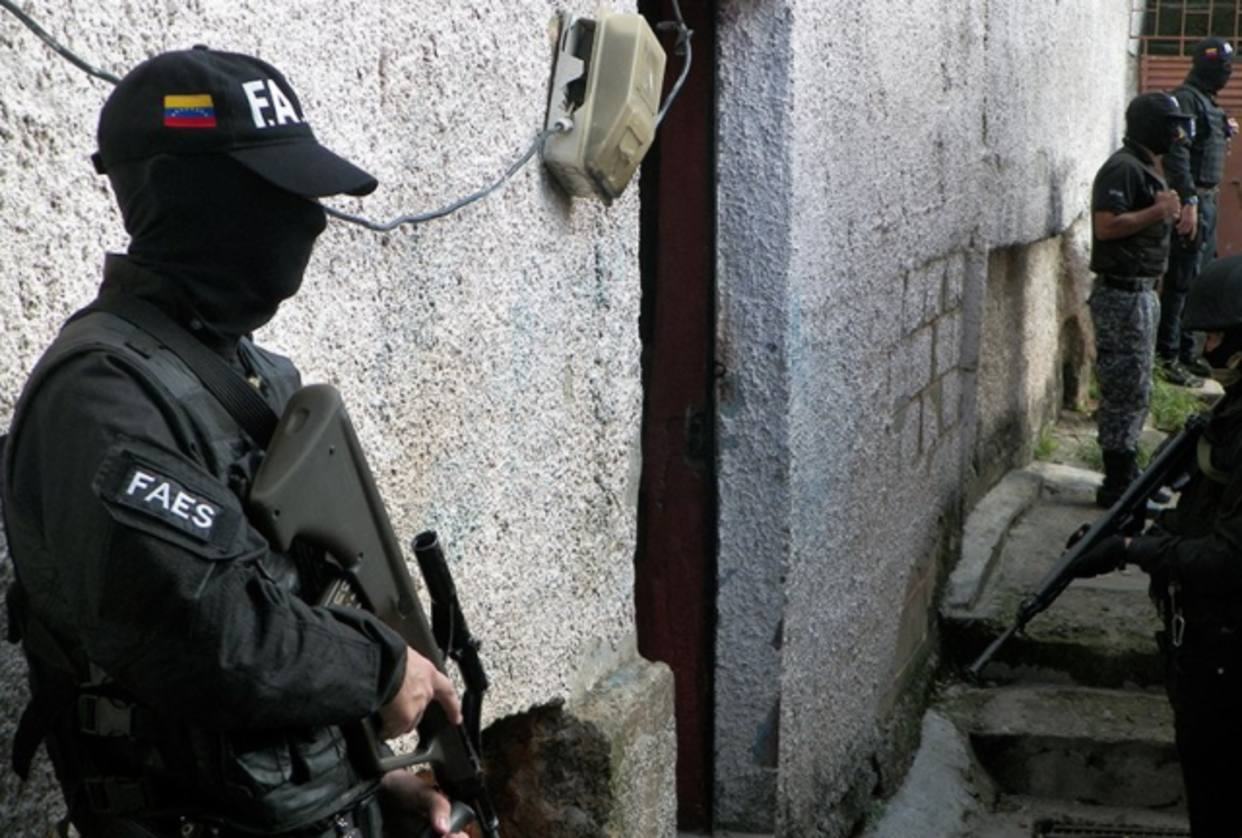
\includegraphics[width=300px]{120.jpg}%
\newline%
%
El tiro que recibió en la cara el oficial agregado de la PNB José Antonio Canales Alemán dio origen al operativo en la Torre Viasa, en Candelaria, por parte de la FAES al mediodía del lunes en la avenida Bolívar. El procedimiento causó siete muertos. Alguien dijo que los autores de la lesión ocasionada al policía se refugiaron en la torre.%
\newline%
%
Uno de los fallecidos es Asley José Flores Rodríguez, de 41 años de edad, padre de un adolescente de 16 años de edad. Flores Rodríguez estaba a presentación ante un tribunal; formaba parte de una cooperativa, integrada por 20 habitantes de la torre, que se dedica a la fabricación de tostones que venden a mayoristas.%
\newline%
%
Flores Rodríguez estaba rallando plátanos en su apartamento del piso 10. Un familiar dijo que los hombres fueron llevados a la planta baja donde apartaron a los adolescentes y dejaron a quienes estaban a presentación y tenían antecedentes; luego fueron llevados al piso 11 donde los mataron. “Cada 5 minutos mataban a uno. No hubo enfrentamiento”, indicó el pariente. Mujeres y niños fueron confinados en los apartamentos y no les permitieron salir.%
\newline%
%
Los fallecidos fueron identificados como Johan Alberto Mijares Izquiel, de 22 años de edad; Vladimir de Jesús González García, con registro por porte y ocultamiento de arma de fuego; Asley José Flores Rodríguez, por el mismo delito; Jhoanni José Roca Gil, de 35 años de edad, solicitado, pero no se indica el delito, y Alexis Richard Lozada, de 31 años de edad. Otros dos fueron identificados con los alias del Guajiro y el Negro. La familia de Roca Gil, técnico de teléfonos y evangélico de la iglesia Jesucristo la Gloria Eterna, dijo que este era padre de tres niños.%
\newline%
%
Otro hombre a quien mataron en el piso 11 fue identificado como Davinson Fernández Maiz. Conocidos no precisaron su edad, pero dijeron que era un joven que se ganaba la vida con la fabricación y venta de tostones. “Y a los que tenían contra la pared eran amenazados por los policías, que tenían drogas en las manos y decían que se las iban a sembrar”, expresaron vecinos.%
\newline%
%
También robaron.~“Fueron ejecuciones a sangre fría. No les importó que había niños, personas con alguna discapacidad”, manifestó una mujer, que prefirió reservar su identidad por temor a represalias. Indicó que luego del operativo, al que muchos calificaron como “la masacre de la Torre Viasa”, los vecinos se solidarizaron con familias que posteriormente fueron a reclamar los cuerpos de sus hijos, yernos, hermanos o esposos en el Hospital Vargas, en Caracas, y ~después en la morgue de Bello Monte.%
\newline%
%
Los niños quedaron al cuidado de otras personas, mientras que el resto organizaba sus enseres en las oficinas de la torre, de 14 pisos, que desde 2006 se convirtieron en apartamentos improvisados con el permiso otorgado por el entonces alcalde mayor de Caracas, Juan Barreto, con la promesa de ser reubicados en urbanismos fuera de la capital.%
\newline%
%
Iluminados con linternas y hasta ayer en la madrugada, los ocupantes dedicaron el tiempo para reorganizar los destrozos ocasionados y así notaron que los funcionarios también robaron desde dinero en efectivo, equipos tecnológicos, comida, pañales, hasta ropa y otros enseres de valor. “Se llevaron hasta la leche de mi hijo de meses”, denunció Carolina Mendoza.%
\newline%
%
Durante el operativo se habrían incautado cuatro pistolas, una escopeta calibre 12 y dos revólveres, según fuentes de La FAES; sin embargo, residentes de la torre negaron la existencia de armas o drogas.%
\newline%
%
\end{document}